\section{User Centred Studies} \label{sec:user-studies}

Developing a robot for aged people brings some delicate questions.
The potential users sometimes have few, or nonexistent, experience with technology, which makes it is difficult for them to understand how robots work and what they can actually do.

Considering the goal of developing a social embodied agent in the game scenario, user studies will be required, similarly to what Pereira et al. have done with the Risk player.
These user studies aim to collect specific social, verbal and nonverbal behaviours, and also some cognitive and strategic guidelines in the domain of \emph{Sueca}.
Additionally, another goal of these user studies is to understand their needs, expectations, and fears \cite{Oliveira}. As a result, the following pilot study was developed in a care home in order to answer all these questions.
It involved two different activities, a focus group and a card game as a result of two distinct motivations, understanding the elderly' concerns about robots and collecting information in the game domain.





\subsection{Focus Group}
The focus group firstly aimed to introduce the team.
It is important to establish a connection with this care home for further studies.
This kind of user study also seems to be a good approach for a first meeting due to the informal and conversational way of interacting with them.
Usually, people tend to feel comfortable and easily share their opinions about the topic being discussed.

\subsubsection{Methodology}
The elderly participants were divided into groups of 5 people.
There were 2 researchers per group commanding and guiding all the process.
The list of materials used, per group:

\begin{itemize}
\item A video to illustrate what is a robot;
\item Photographies of different robots (including the service and companion types);
\item Two white boards and three pens (black, red and green);
\item Three hypothetical stories of robots;
\item An audio recorder;
\item Four lavalier microphones;
\item A video camera.
\end{itemize}

The last two items were only used for a further analysis of this focus group.
The video tries to answer the questions: what is a robot, what can robots do, how do they work, do they fail and how do science fiction movies present robots to us.
In order not to bias their thoughts, we tried to gather positive and negative aspects of existing robots.
The three hypothetical stories aim to bring ethical discussions to the focus group.
For instance, an elderly that owns a robot in his home tells him a secret.
If that robot is questioned about the secret, should it or should it not tell other people the truth?

\subsubsection{Procedures}
All the materials enumerated in the previous list were arranged as in Figure~\ref{fig:focus-group}.
Firstly, each person in the room briefly introduces himself in order to make everyone feeling more comfortable.
Secondly, the video is shown.
Then, everyone starts discussing about robots' purposes and they are registered in one of the white boards with the black coloured pen.
People also express a positive or negative impression of each robot's purpose and their opinions decide the colour of the surrounding line.
For instance, the sentence ``Call an ambulance'' written on the board is surrounded by a green line if they think it is a good purpose for a robot.
After finishing this task, one of the group leaders writes all the sentences previously collected in the second board but without the surrounding green or red lines.
The other group leader starts reading the hypothetical stories and opens a new discussion about what the robots of each story should do.
He also presents the photographs and tries to understand which robot is more suitable for each purpose in their opinion.
When bringing the new board to the room, the idea is to understand if their positive and negative opinions about each purpose have changed.

\begin{figure}
        \centering
        \begin{subfigure}[h]{0.49\textwidth}
                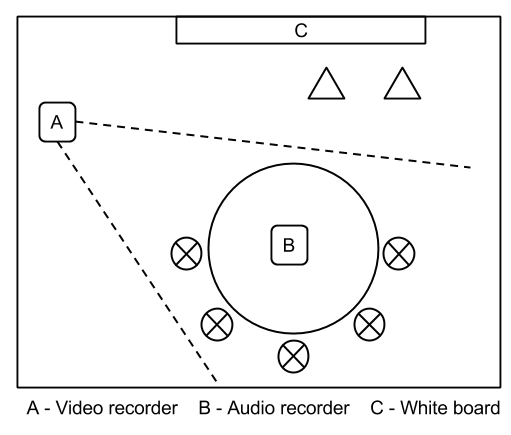
\includegraphics[width=\textwidth]{./img/focusGroup}
                \caption{Focus Group}
                \label{fig:focus-group}
        \end{subfigure}
        \begin{subfigure}[h]{0.49\textwidth}
                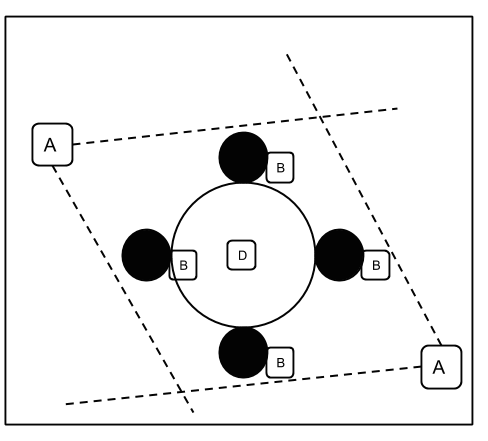
\includegraphics[width=\textwidth]{./img/cardGame}
                \caption{Card game}
                \label{fig:card-game}
        \end{subfigure}
        \caption{Setting of the user study activities. \textbf{A} - Video recorder \textbf{B} - Audio recorder / Microphone \textbf{C} - White board \textbf{D} - cards \ding{108} - Aged person \ding{115} - Group leader}\label{fig:user-studies}
\end{figure}


\subsubsection{Preliminary Results}

This focus group is an ongoing activity that has not yet been fully analysed.
Information has already been collected from 3 different focus groups with a sum of 15 participants.
For instance, contrasting with what was expected, the elderly do not feel uncomfortable and disrespected with a robot calling the doctor and revealing improper behaviours about its owner.
Instead, they think it is a valuable aid in their lives and might save them while disrespecting strict instructions.
In addition, their safety is their prior worry.
When walking through the house and sometimes due to physical disabilities, they fear about falling and not being noticed.







\subsection{Card Game}
This pilot card game activity aims two distinct purposes.
On one hand, to collect all kind of behaviours and interactions between players during the game.
On the other hand, to rehearse and check the technical set-up for further studies.
It is important to understand difficulties, for instance, lightning conditions might affect video recording, or the room acoustic and noise might affect audio recording.
Testing these conditions is essential to guarantee the analyses of additional studies.
Moreover, this activity aims to perceive how the elderly play, what they say and how they behave in certain game states.

\subsubsection{Methodology}
Recording each \emph{Sueca} card game requires four players, a card deck, a table and chairs for the four players, two video cameras and an audio recorder with four microphones.

\subsubsection{Procedures}
All the previously enumerated material was arranged as in the Figure~\ref{fig:card-game}.
Each video camera was positioned to capture the hands of two adjacent players.
Players were recorded during a tournament of several games.
They were told to play as long as they wanted with a maximum duration of one hour.

\subsubsection{Preliminary Results}
The session took only 40 minutes, since the 4 players were feeling weary.
Ten games, with an average duration of 3,75' each, were collected.
From the average duration, 1' belongs to the initial setting of shuffling, distributing, and rearranging the cards in each hand.
The points per team were being counted during the game.

As expected, players did not frequently talk during the game.
\emph{Sueca} is indeed traditionally called a silent game.
After a game, paired players frequently discuss extremely good or bad moves from each other.
However, the analysis was focused mostly on interactions during the game.
Table~\ref{tab:interactions} illustrates the collected expressions, the game stage and its intention.
Considering players said specific domain words, expressions were not translated in order not to lose their meaning and regarding the future usage of these sentences in a Portuguese environment.


\begin{table}[h]
\caption{Examples of expressions collected during the card game activity and its respective classification.}
\resizebox{\textwidth}{!}{%
\begin{tabular}{|l|m{0.3\textwidth}|m{0.3\textwidth}|}
\hline
\textbf{Expression} & \textbf{Game Stage} & \textbf{Intention} \\ \hline
\textit{Joga }{[}player-name{]}\textit{!} & Before a play & Speed up a play. \\ \hline
\textit{Anda }{[}player-name{]}\textit{!} & Before a play & Speed up a play. \\ \hline
\textit{Podes jogar, }{[}player-name{]}\textit{!} & Before a play & Speed up a play. \\ \hline
\textit{Quase que livr\'amos.} & After collecting the first points & Hopeful/ironic comment. \\ \hline
\textit{E eu puxo trunfo.} & Initialising a turn with a trump card & State an action. \\ \hline
Outro trunfo! & Play a trump card after an already played trump card & State an action. \\ \hline
\textit{Outro(a) }{[}suit{]}\textit{!} & Play a {[}suit{]} card after an already played {[}suit{]} card & State an action. \\ \hline
\textit{O trunfo \'e }{[}suit{]}\textit{.} & Anytime & Give game information. Answer a question. \\ \hline
\end{tabular}
}
\label{tab:interactions}
\end{table}


Regarding the video recording, a relevant aspect that has been noticed was the lighting reflection through the cards.
If this technique will be adopted to collect game play information, lighting conditions should be well prepared.


%Additional cues will be evaluated 







